

% \documentclass[article,tikz,border=3mm]{standalone}
\documentclass{article}
\usepackage{blindtext}

% setting up the margin of the paper 
\usepackage[a4paper, total={6.5in, 9in}]{geometry}

% setup for font family for the title/section name, for text font you have set ti seperately
\usepackage[T1]{fontenc}
\usepackage{lmodern}

% package for tables, this package I don't why always stay at the top of the document
\usepackage{tikz}
% I don't know what is this for right now
\usepackage{mathtools,eqparbox}

% not sure for right now 
\usepackage{array}

% index package 
\usepackage{imakeidx}
\makeindex % this line is mandatory

% package for basic symbol characters $/rhd$
% https://artofproblemsolving.com/wiki/index.php/LaTeX:Symbols
\usepackage{latexsym}

% system of equation (such as large bracket)
\usepackage{amsmath}
\usepackage[makeroom]{cancel} % cancel out single item by using \cancel{}
\usepackage{soul} % straight cross line not in matrix
\usepackage{nicematrix} % draw straight cross line inside matrix
\usepackage{mathtools} % display fraction-like 
\newcommand\aug{\fboxsep=-\fboxrule\!\!\!\fbox{\strut}\!\!\!} % this line is for the veritical line in augmented matrix, but you can use array to achieve this as well

\usepackage{pgfplots} % 2 dimensional ploting
\pgfplotsset{compat=1.10}
\usetikzlibrary{datavisualization.formats.functions} % 2 dimensional ploting

\usepackage{tikz-3dplot} % 3 dimensional plot

% ================================================== Main.tex ==============================================
\begin{document}


% ploting the table using tikz package
\begin{table}
\[\begin{array}{c|ccccc}
\tikz{\node[below left, inner sep=1pt] (food) {Food};%
      \node[above right,inner sep=1pt] (ingredient) {Ingredient};%
      \draw (food.north west|-ingredient.north west) -- (food.south east-|ingredient.south east);}
 & Ca^{2+} & Na^{+} & Sugar & Calories \\
\hline
    rice & x_{11} & x_{12} & x_{13} & y_{1} \\
    meat & x_{21} & x_{22} & x_{23} & y_{2} \\
    fish & x_{31} & x_{32} & x_{33} & y_{3} \\
    apple & x_{41} & x_{42} & x_{43} & y_{4} \\
\end{array}\]
\caption{Nutrition Values}
\end{table}

% section start
\section{Representation of Matrix}
Table could be viewed as a matrix, below are an illustration coressponding to the above table. The 4x3 matrix stands for attributes while weights are used for calculating y (outcome)
\begin{center}
    $\begin{bmatrix}
        x_{11} & x_{12} & x_{13} \\
        x_{21} & x_{22} & x_{23} \\
        x_{31} & x_{32} & x_{33} \\
        x_{41} & x_{42} & x_{43} \\
    \end{bmatrix}$
    x 
    $\begin{bmatrix} 
        w_{1} \\ 
        w_{2} \\
        w_{3} \\
    \end{bmatrix}$
    =
    $\begin{bmatrix} 
        y_{1} \\ 
        y_{2} \\
        y_{3} \\
        y_{4} \\
    \end{bmatrix}$ \\
\end{center}

% only centering centain text
\centerline{matrix multiplication(dim): 4x3 • 3x1 = 4x1}

% subsection
\subsection{In general}
\text{Like numbers, matrices can be added, subtracted, multiplied, and divided} \\
\text{matrices have many other uses in mathematics and the sciences, knowing matrix algebra is essential}

% new section 
\section{Matrix Properties}
\subsection{Equality}
The matrices A = $[a_{ij}]$ and B = $[b_{ij}]$ are equal if and only if \\ 
• they have the same dimension m x n \\ 
• corresponding entries are equal $a_{ij} = b_{ij}$: for i=1, 2, ... ,m and j=1, 2, ... ,n 


% stretch the size of the table in vertical level
\begin{center}
    \renewcommand{\arraystretch}{4}

    \begin{tabular}{|*2{>{\renewcommand{\arraystretch}{1}}c|}}
    \hline
    \textbf{Equal} & \textbf{Unequal}\\
    \hline
    $ \left[ \begin{array}{ccc} \sqrt{4} & 2^2 & e^0 \\ 0.5 & 1 & 1-1 \end{array}\right]$ = $ \left[ \begin{array}{ccc} 2 & 4 & 1 \\ \frac{1}{2} & \frac{2}{2} & 0 \end{array}\right]$  & 
    $ \left[ \begin{array}{cc} 1 & 2 \\ 3 & 4 \\ 5 & 6 \end{array}\right]$ $\neq \left[ \begin{array}{ccc} 1 & 3 & 5 \\ 2 & 4 & 6 \end{array}\right]$ \\
    \hline
    \end{tabular} 
\end{center}

• Find a, b, c, and d if 
$\begin{bmatrix}
    a & b \\ 
    c & d
\end{bmatrix}$
= 
$\begin{bmatrix}
    1 & 3 \\ 
    5 & 2
\end{bmatrix}$. 
In order for two matrices to be equal, we have a=1, b=3, c=5, d=2


\subsection{Addition, Subtraction, and Scalar Multiplication}

Let A = $[a_{ij}]$ and B = $[b_{ij}]$ be matrices of the \textbf{same dimension} m x n, c be any real number \\
\indent 1) addition: A + B = $[a_{ij} + b_{ij}]$ \\
\indent 2) subtraction: A - B = $[a_{ij} - b_{ij}]$ \\ 
\indent 3) scalar product: cA = $[ca_{ij}]$

\subsection{Multiplcation of Matrices}
The product AB (or A•B) of two matrices A and B is defined only when the number of columns in A is equal to the number of rows in B 



\begin{center}
  \begin{tabular}{ | l | c | r |}
    \hline
    Matrices & A & B \\ \hline
    Dimensions & m x \textbf{n} & \textbf{n} x k \\ 
    \hline
  \end{tabular} \\
\end{center}
\centerline{n is the columns in A, rows in B, the new resulting matrix has the dimension of \textbf{m x k}} 

\begin{itemize}
    \item[$>>$] \textbf{Inner Product} \\
    if $[a_1 a_2 \hdots a_n]$ is a row of A, and if 
    $\begin{bmatrix} 
        b_1 \\ 
        b_2 \\ 
        \vdots \\
        b_n \\
    \end{bmatrix}$
    is a column of B, their inner product is the number \\ $\mathbf{a_1b_1 + a_2b_2 + \hdots + a_nb_n}$

    \item[$>>$] \textbf{ex)} \\ 
    $\begin{bmatrix} 
        2 & -1 & 0 & 4
    \end{bmatrix}$
    and 
    $\begin{bmatrix} 
        5 \\ 
        4 \\ 
        -3 \\
        \frac{1}{2} \\
    \end{bmatrix}$
    gives: 2•5 + (-1)•4 + 0•(-3) + 4• $\frac{1}{2}$ = 8

    \item[$>>$] $\mathbf{c_{ij}}$ \\ 
    based on the examples, the resulting formula for matrices multiplcation with multi-entry

    $\begin{bmatrix} 
        a_{11} & a_{12} \\ 
        a_{21} & a_{22} \\ 
    \end{bmatrix}$
    • 
    $\begin{bmatrix} 
        b_{11} & b_{12} & b_{13} \\ 
        b_{21} & b_{22} & b_{23} \\ 
    \end{bmatrix}$
    = \\
    $\begin{bmatrix} 
        c_{11}(a_{11}*b_{11} + a_{12}*b_{21}) & c_{12}(a_{11}*b_{12} + a_{12}*b_{22}) & c_{13}(a_{11}*b_{13} + a_{12}*b_{23}) \\ 
        c_{21}(a_{21}*b_{11} + a_{22}*b_{21}) & c_{22}(a_{21}*b_{12} + a_{22}*b_{22}) & c_{23}(a_{21}*b_{13} + a_{12}*b_{23}) \\ 
    \end{bmatrix}$

\end{itemize}


\subsection{Properties of Matrix Multiplication}

$\rhd$ Order Matters \\
\indent 1) $A^2 - B^2 = (A+B)(A-B)$ {\color{red}False: expand and do the calculation}  \\
\indent 2) $(A+B)^2 = A^2 + 2AB + B^2$ {\color{red}False: found order changed after expanding} \\
\indent 3) $(A-B)^2 = A^2 - 2AB + B^2$ {\color{red}False: found order changed after expanding}  \\
\indent 4) $(AB)^2 = A^2B^2$ {\color{red}False: (AB)(AB) = ABAB, there is BA discomfort with original order} \\
\indent 5) $(kA)(kB) = k^2(AB)$ {\color{green}True}


\subsection{Application of Matrix Multiplcation}

$\begin{bmatrix} 
    1 & -1 & 3 \\ 
    1 & 2 & -2 \\ 
    3 & -2 & 5 \\ 
\end{bmatrix}$
• 
$\begin{bmatrix} 
    x \\
    y \\ 
    z \\
\end{bmatrix}$
= 
$\begin{bmatrix} 
    4 \\
    10 \\ 
    14 \\
\end{bmatrix}$
becomes this
$\begin{bmatrix} 
    x & -y & 3z \\ 
    x & 2y & -2z \\ 
    3x & -y & 5z \\ 
\end{bmatrix}$
=
$\begin{bmatrix} 
    4 \\
    10 \\ 
    14 \\
\end{bmatrix}$
\\
\textbf{it becomes the system of linear equation}
$\begin{cases}
    x-y+3z = 4 \\ 
    x+2y-2z = 10 \\ 
    3x-y+5z = 14 \\ 
\end{cases}$

% ------------ different way of writing system of equation -------------
% \begin{equation*}
%   \left\{
%     \begin{aligned}
%       & x-y+3z = 4 \\
%       & x+2y-2z = 10 \\
%       & 3x-y+5z = 14 \\
%       % & {\left|
%       %   \frac{k_{p\omega}s + k_{i\omega}}{s} \cdot \frac{1}{Ts + 1}
%       % \right|}_{s = j \cdot 2\pi} = 1
%     \end{aligned}
%   \right.
% \end{equation*}
% ----------------------------------------------------------------------


\subsection{Matrix Transpose}

1) A: $\begin{bmatrix} x_1 & x_2 & x_3 \end{bmatrix}$ is a 1x3 matrix $\rightarrow$ $A^T$: $\begin{bmatrix} x_1 \\ x_2 \\ x_3 \end{bmatrix}$ becomes a 3x1 matrix \\
2) A square Matrix A is symmetric if x = $x^T$, visual representation: $\begin{bmatrix} a & b \\ c & d \end{bmatrix} \rightarrow$ $\begin{bmatrix} a & c\\ b & d \end{bmatrix}$\\
3) A = $\begin{bmatrix} 1 & 5 \\ 5 & 1 \end{bmatrix}$ = $A^T$ = $\begin{bmatrix} 1 & 5 \\ 5 & 1 \end{bmatrix}$ \\
4) matrix operation with transpose: $\begin{cases} (A^T)^T = A \\ (A+B)^T = A^T + B^T \\ (AB)^T = B^TA^T \\ (cA)^T = c(A^T) \end{cases}$




\section{Determinants}

If a matrix is square (rows = columns), then we can assign to it a number called its determinant. \\ 
\indent >> determinant can be used to solve systems of linear equation \\
\indent >> useful in determining whether a matrix has an inversse \\ 
\indent >> denote by det(A) or |A|

\subsection{Determinants of 2 x 2 Matrix}
A = $\begin{bmatrix} a & b \\ c & d \end{bmatrix}$ is: det(A)= $\begin{vmatrix} a & b \\ c & d \end{vmatrix}$ = ad - bc \\ 
B = $\begin{vmatrix} 6 & -3 \\ 2 & 3 \end{vmatrix}$, det(B) = 6•3-(-3)•2 = 18 -(-6) = 24


\subsection{Determinants of n x n Matrix}
If A is an n x n matrix, the determinant of A is obtained by multiplying each element of the first row by its cofactor, and then adding the result, below is the general form 
\begin{itemize}

    \item[>>] cofactor: the determinant for chosen element with row and column are crossed out(denoted by $a_{ij}$)
    \item[>>] GF => expand the first row: det(A)=|A|= $\begin{vmatrix}
                                        a_{11} & a_{12} & \hdots & a_{1n} \\ 
                                        a_{21} & a_{22} & \hdots & a_{2n} \\
                                        \vdots & \vdots & \ddots & \vdots \\
                                        a_{n1} & a_{n2} & \hdots & a_{nn}
                                    \end{vmatrix} = a_{11}A_{11} + a_{12}A_{12} + \hdots + a_{1n}A_{1n}$ 
    \item[>>] use 3x3 matrix as example: A = $\begin{vmatrix} 2 & 3 & -1 \\ 0 & 2 & 4 \\ -2 & 5 & 6 \end{vmatrix}$ while the positive and negative sign of $a_{ij}$ 
              is determined by checking the odd or even of (i+j), like this $\begin{bmatrix} + & - & +  \\ - & + & - \\ + & - & + \end{bmatrix}$
    \item[>>] expand the first row
    \begin{itemize}
        \item[1)] $A_{11}$ = 2
            $\begin{pNiceMatrix} 
                  2 & 3 & -1 \\ 
                  0 & 2 & 4 \\ 
                  -2 & 5 & 6 
                  \CodeAfter 
                  \begin{tikzpicture}
                     \draw [thick,red] (1-1.west) -- (1-3.east); 
                     \draw [thick,red] (1-1.north) -- (3-1.south); 
                  \end{tikzpicture}
              \end{pNiceMatrix}$
              = 2 $\begin{vmatrix} 2 & 4 \\ 5 & 6 \end{vmatrix}$

        \item[2)] $A_{12}$ = -3  
              $\begin{pNiceMatrix}
                  2 & 3 & -1 \\ 
                  0 & 2 & 4 \\ 
                  -2 & 5 & 6 
                  \CodeAfter 
                  \begin{tikzpicture}
                     \draw [thick,red] (1-1.west) -- (1-3.east); 
                     \draw [thick,red] (1-2.north) -- (3-2.south); 
                  \end{tikzpicture}
              \end{pNiceMatrix}$
              = -3 $\begin{vmatrix} 0 & 4 \\ -2 & 6 \end{vmatrix}$

        \item[3)] $A_{12}$ = -3  
              $\begin{pNiceMatrix}
                  2 & 3 & -1 \\ 
                  0 & 2 & 4 \\ 
                  -2 & 5 & 6 
                  \CodeAfter 
                  \begin{tikzpicture}
                     \draw [thick,red] (1-1.west) -- (1-3.east); 
                     \draw [thick,red] (1-3.north) -- (3-3.south); 
                  \end{tikzpicture}
              \end{pNiceMatrix}$
              = -1 $\begin{vmatrix} 0 & 2 \\ -2 & 5 \end{vmatrix}$
    \end{itemize}

    det(A) = 2(2•6 - 4•5) -3[0•6-4(-2)] -[0•5-2(-2)] \\ 
    = -16-24-4 \\
    = -44

    \item[>>] you can expand a whole row or column in either direction, not only the first row, you can also use the last column something like that -> Same result.
\end{itemize}

\subsection{invertibility}
if A is a square matrix, then A has an inverse if and only if det(A) $\neq$ 0 \\
\indent >> ex. show that the matrix A has no inverse A=$\begin{bmatrix} 1 & 2 & 0 & 4  \\ 0 & 0 & 0 & 3 \\ 5 & 6 & 2 & 6 \\ 2 & 4 & 0 & 9\end{bmatrix} = 
-0 \times A_{21} + 0 \times A_{22} - 0 \times A_{23} + 3 \times A_{24} = 3A_{24} = 3 \begin{vmatrix} 1 & 2 & 0 \\ 5 & 6 & 2 \\ 2 & 4 & 0 \end{vmatrix} = 3(-2) \begin{vmatrix} 1 & 2 \\ 2 & 4 \end{vmatrix}
3(-2)(1 \times 4-2 \times 2) = 0$

\indent >> since the determinant = zero, so the matrix doesn't have an inverse 

\indent >> usually we span the first row for calculating determinants of matrix that is greater than 2 dimensions with nested operation, 
but you can do that will any rows or columns as long as it is the consistent row/column for nested operations, choose rows/columns with more zeros, which will make the calculation easier


\section{Cramer's Rule}

\indent The solutions of linear equations can sometimes be expressed using determinants, refer to the following example 

\indent >> $\begin{cases} ax + by = r \\ cx + dy = s \end{cases}$ solve the this for the variable x.

\indent >> To elimninate the varible y, we multiply the first equation by d and the second by b, and subtract: 
\begin{align*} adx + bdy = rd \\ bcx + bdy = bs \\ \mathclap{\rule{6cm}{0.3pt}}\\ adx-bcx = rd-bs \end{align*}

\indent >> assume that ad-bc $\neq$ 0, we can now solve this equation for x: $x = \frac{rd-bs}{ad-bc}$, and for y: $y = \frac{as-cr}{ad-bc}$
\indent >> since the numerator and denominator of the fractions for x and y are determinants of 2 x 2 matrices, so we can express in the following way: \\
$\begin{cases}  ax + by = r \\ cx + dy = s \end{cases}$ has the solution $x = \frac{\begin{vmatrix} r & b \\ s & d \end{vmatrix}}{\begin{vmatrix} a & b \\ c & d \end{vmatrix}}, 
y = \frac{\begin{vmatrix} a & r \\ c & s \end{vmatrix}}{\begin{vmatrix} a & b \\ c & d \end{vmatrix}},$ provided $\begin{vmatrix} a & b \\ c & d \end{vmatrix} \neq 0$

\indent >> Cramer's Rule: $D = \begin{bmatrix} a & b \\ c & d \end{bmatrix}$, $D_x = \begin{bmatrix} r & b \\ s & d \end{bmatrix}$, $D_y = \begin{bmatrix} a & r \\ c & s \end{bmatrix}$. 
The solution can be written as: $x = \frac{|D_x|}{|D|}$ and $y = \frac{|D_y|}{|D|}$

\indent >> ex. solve the following system using Cramer's Rule: $\begin{cases} 2x + 6y = -1(r) \\ x + 8y = 2(s) \end{cases}$

\begin{center}
    $|D| = \begin{vmatrix} 2 & 6 \\ 1 & 8 \end{vmatrix} = 2 \cdot 8 - 6 \cdot 1 = 10$  \\ 
    $|D_x| = \begin{vmatrix} -1 & 6 \\ 2 & 8 \end{vmatrix} = (-1) \cdot 8 - 6 \cdot 2 = -20$ \\ 
    $|D_y| = \begin{vmatrix} 2 & -1 \\ 1 & 2 \end{vmatrix} = 2 \cdot 2 - (-1) \cdot 1 = 5$
\end{center}

\indent >> the solution is $x = \frac{|D_x|}{|D|} = \frac{-20}{20} = -2$ and $y = \frac{|D_y|}{|D|} = \frac{5}{10} = \frac{1}{2}$


\section{Inverse of the Matrix}
A square matrix M is invertible or non-singlar if there exist a matrix B such that A•B = I

\subsection{Identity Matrix}
In linear algebra, the \textbf{identity matrix} of size n is the n x n \textbf{square matrix} with \textbf{ones} on the \textbf{main diagonal} and \textbf{zeros} elsewhere, denoted by $I_n$ \\
\indent >> $I_1$=[1], $I_2=\begin{bmatrix} 1 & 0 \\ 0 & 1 \end{bmatrix}$, $I_3=\begin{bmatrix} 1 & 0 & 0 \\ 0 & 1 & 0 \\ 0 & 0 & 1 \end{bmatrix}$, $\hdots$ ,
$I_n=\begin{bmatrix} 1 & 0 & 0 & \hdots & 0 \\ 0 & 1 & 0 & \hdots & 0 \\ 0 & 0 & 1 & \hdots & 0 \\ \vdots & \vdots & \vdots & \ddots & \vdots \\ 0 & 0 & 0 & \hdots & 1 \end{bmatrix}$


\indent >> A = $\begin{bmatrix} 2 & 1 \\ 5 & 3 \end{bmatrix}$, B = $\begin{bmatrix} 3 & -1 \\ -5 & 2 \end{bmatrix}$, verify the inverse of a matrix (both AB = I and BA = I)\\ 
\indent A $\cdot$ B = $\begin{bmatrix} 2 & 1 \\ 5 & 3 \end{bmatrix} \cdot \begin{bmatrix} 3 & -1 \\ -5 & 2 \end{bmatrix} = 
\begin{bmatrix} 2 \cdot 3 + 1(-5) & 2(-1) + 1 \cdot 2 \\ 5 \cdot 3 + 3(-5) & 5(-1) + 3 \cdot 2 \end{bmatrix} = \begin{bmatrix} 1 & 0 \\ 0 & 1 \end{bmatrix}$


\subsection{Inverse of 2 x 2 Matrix}

If A = $\begin{bmatrix} a & b \\ c & d \end{bmatrix}$, then $A^{-1} = \frac{1}{ad - bc} \begin{bmatrix} d & -b \\ -c & a \end{bmatrix}$, remember to verify that $AA^{-1} = A^{-1}A = I$

\subsection{Inverse of n x n Matrix}

Let A be the matrix A $\begin{bmatrix} 1 & -2 & -4 \\ 2 & -3 & -6 \\ -3 & 6 & 15 \end{bmatrix}$. (a) Find $A^{-1}$. (b) Verify that $AA^{-1} = A^{-1}A = I$.

\indent a).
\begin{align*} 
\left(
\begin{array}{rrr|rrr} 
    1 & -2 & -4 & 1 & 0 & 0 \\ 
    2 & -3 & -6 & 0 & 1 & 0 \\
    -3 & 6 & 15 & 0 & 0 & 1 \\ 
\end{array}
\right)
&\xrightarrow[R_3+3R_1 \to R_3]{R_2-2R_1 \to R_2} 
\left(
\begin{array}{rrr|rrr} 
    1 & -2 & -4 & 1 & 0 & 0 \\ 
    0 & 1 & 2 & -2 & 1 & 0 \\
    0 & 0 & 3 & 3 & 0 & 1 \\ 
\end{array}
\right) \\[5pt]
&\xrightarrow{\frac{1}{3}R_3 \to R_3} 
\left(
\begin{array}{rrr|rrr} 
    1 & -2 & -4 & 1 & 0 & 0 \\ 
    0 & 1 & 2 & -2 & 1 & 0 \\
    0 & 0 & 1 & 1 & 0 & \frac{1}{3} \\ 
\end{array}
\right) \\[5pt]
&\xrightarrow{R_1+2R_2 \to R_1}
\left(
\begin{array}{rrr|rrr} 
    1 & 0 & 0 & -3 & 2 & 0 \\ 
    0 & 1 & 2 & -2 & 1 & 0 \\
    0 & 0 & 1 & 1 & 0 & \frac{1}{3} \\ 
\end{array}
\right) \\[5pt]
&\xrightarrow{R_2-2R_3 \to R_2}
\left(
\begin{array}{rrr|rrr} 
    1 & 0 & 0 & -3 & 2 & 0 \\ 
    0 & 1 & 0 & -4 & 1 & -\frac{2}{3} \\[2pt]
    0 & 0 & 1 & 1 & 0 & \frac{1}{3} \\ 
\end{array}
\right)
\end{align*}

\indent b). solve yourself

\section{Gaussian Elimination}
In general, to solve a system of linear equations using its \textbf{augmented matrix}, we use \textbf{elementary row operations} to arrive at a matrix in a certain form. \\
1) row-echelon form \\ 
2) reduced row-echelon 

\subsection{\underline{Row-Echelon} and \underline{Reduced Row-Echelon Form}}
A matrix is in row-echelon form if it satisfies the following conditions:
\begin{itemize}
    \item[1)] The first nonzero number in each row (reading from left to right) is 1. This is called the leading entry 
    \item[2)] The leading entry in each row is to the right of the leading entry in the row immediately above it
    \item[3)] All rows consisting entirely of zeros are at the bottom of the matrix
\end{itemize}
A matrix is in reduced row-echelon form if it is in row-echelon form, and also satisfies the following condition. 
\begin{itemize}
    \item[4)] Eveny number above and below each leading entry is a 0
\end{itemize}


\newcommand{\sunderb}[2]{
  \mathclap{\underbrace{\makebox[#1]{$\cdots$}}_{#2}}
}


\subsection{Not in Row-Echelon Form}

\begin{center}
$\begin{bNiceArray}{cccc|c}[right-margin=.4em]
    0 & \color{red}1 & -\frac{1}{2} & 0 & 7 \\ 
    \color{red}1 & 0 & 3 & 4 & -5 \\
    0 & 0 & 0 &\color{red}1 & 0.4 \\
    0 & \color{red}1 & 1 & 0 & 0 \\ 
    \CodeAfter 
    \UnderBrace[shorten,yshift=3pt]{4-1}{4-4}{\text{Leading 1's do not shift to the right in successive rows}}
\end{bNiceArray}$
\end{center}


\subsection{Correct Form}
\begin{center}
    \renewcommand{\arraystretch}{4}

    \begin{tabular}{|*2{>{\renewcommand{\arraystretch}{1}}c|}}
    \hline
    \textbf{Row-Echelon Form} & \textbf{Reduced Row-Echelon Form}\\
    \hline
    $ \left[ \begin{array}{ccccc} 
        \color{red}1 & 3 & -6 & 10 & 0 \\ 
        0 & 0 & \color{red}1 & 4 & -3 \\ 
        0 & 0 & 0 & \color{red}1 & \frac{1}{2} \\
        0 & 0 & 0 & 0 & 0
    \end{array}\right]$ & 
    $ \left[ \begin{array}{ccccc}
        \color{red}1 & 3 & 0 & 0 & 0 \\
        0 & 0 & \color{red}1 & 0 & -3 \\
        0 & 0 & 0 & \color{red}1 & \frac{1}{2} \\ 
        0 & 0 & 0 & 0 & 0 
    \end{array}\right]$  \\
    \hline
    \text{leading 1's shift to the right in successive rows} & \text{leading 1's have 0's above and below in that column} \\
    \hline
    \end{tabular} 
\end{center}


\subsection{Gaussian Elimination}
Once an augmented matrix is in row-echelon form, we can solve the corresponding linear system using back-substitution (this technique is called Gaussian Elimination) \\
step 1) Augmented Matrix \\
step 2) Row-Echelon Form \\
step 3) Back-Substitution \\
\indent >> \textbf{complete example:}
$\begin{cases}
    4x + 8y - 4z = 4 \\
    3x + 8y + 5z = -11 \\ 
    -2x + y + 12z = -17
\end{cases}$
first write the augmented matrix of the system, then use elementary row operations to put it in row-echelon form 
\begin{align*} 
\left(
\begin{array}{rrr|r} 
    4 & 8 & -4 & 4 \\ 
    3 & 8 & 5 & -11 \\
    -2 & 1 & 12 & -17 \\ 
\end{array}
\right)
&\xrightarrow{\frac{1}{4}R_1 \to R_1} 
\left(
\begin{array}{rrr|r} 
    \color{red}1 & 2 & -1 & 1 \\ 
    3 & 8 & 5 & -11 \\
    -2 & 1 & 12 & -17 \\ 
\end{array}
\right)
&\xrightarrow[R_3+2R_1 \to R_3]{R_2-3R_1 \to R_2}
\left(
\begin{array}{rrr|r} 
    \color{red}1 & 2 & -1 & 1 \\ 
    \color{red}0 & 2 & 8 & -14 \\
    \color{red}0 & 5 & 10 & -15 \\ 
\end{array}
\right) \\[5pt]
&\xrightarrow{\frac{1}{2}R_2 \to R_2}
\left(
\begin{array}{rrr|r} 
    \color{red}1 & 2 & -1 & 1 \\ 
    \color{red}0 & \color{red}1 & 4 & -7 \\
    \color{red}0 & 5 & 10 & -15 \\ 
\end{array}
\right)
&\xrightarrow{-\frac{1}{10}R_3 \to R_3}
\left(
\begin{array}{rrr|r} 
    \color{red}1 & 2 & -1 & 1 \\ 
    \color{red}0 & \color{red}1 & 4 & -7 \\
    \color{red}0 & \color{red}0 & \color{red}1 & -2 \\ 
\end{array}
\right) \\[5pt]
\end{align*}

\indent >> \textbf{Gauss-Jordan Elimination => Reduced Row-Echelon Form}
\begin{align*}
\left(
\begin{array}{rrr|r} 
    1 & 2 & -1 & 1 \\ 
    0 & 1 & 4 & -7 \\
    0 & 5 & 10 & -15 \\ 
\end{array}
\right)
&\xrightarrow[R_1+R_3 \to R_1]{R_2-4R_3 \to R_2}
\left(
\begin{array}{rrr|r} 
    1 & 2 & \color{red}0 & -1 \\ 
    0 & 1 & \color{red}0 & 1 \\
    0 & 0 & 1 & -2 \\ 
\end{array}
\right)
&\xrightarrow{R_1-2R_2 \to R_1}
\left(
\begin{array}{rrr|r} 
    1 & \color{red}0 & \color{red}0 & -3 \\ 
    0 & 1 & \color{red}0 & 1 \\
    0 & 0 & 1 & -2 \\ 
\end{array}
\right)\\[5pt]
\end{align*}
The solution set becomes: $\begin{cases} x = -3 \\ y = 1 \\ z = -2 \end{cases}$

\section{Inconsistent and Dependent System}
Suppose the augmented matrix of a system of linear equations has been transformed by Gaussian elimination into row-echelon form. Then, exactly one of the following is true:
\begin{itemize}
    \item No Solution 
    \item One Solution 
    \item Infinitely Many Solution
\end{itemize}

\subsection{Inconsistent System(no solution)}
if REF contains \textbf{a row} that represents the equation 0 = c where c is not zero, the system has no solution

\begin{center}
$\begin{vNiceArray}{cccc}[right-margin=.4em]
    1 & 2 & 5 & 7 \\ 
    0 & 1 & 3 & 4 \\
    \color{red}0 & \color{red}0 & \color{red}0 & \color{red}1 \\
    \CodeAfter 
    \UnderBrace[shorten,yshift=3pt]{3-1}{3-4}{\color{red}\text{Last equation says 0 = 1, which impossible at least in my century}}
\end{vNiceArray}$
\end{center} 
$\newline\newline$
\textbf{lines are parallel in n lines are parallel in n dimensons, will never intersect with each other}
\begin{center}
    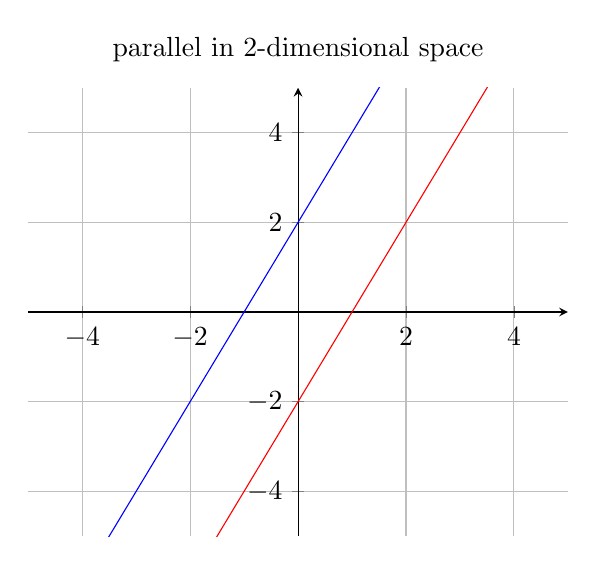
\begin{tikzpicture}
    \begin{axis}[xmin=-5, xmax=5, ymin=-5, ymax=5, axis x line=middle, axis y line=middle, title=parallel in 2-dimensional space, grid=both]
    \addplot[domain=-5:5, color=red]{2*x-2};
    \addplot[domain=-5:5, color=blue]{2*x+2};
    \end{axis}
    \end{tikzpicture}
\end{center}


\subsection{One Solution}
if each variable in the row-echelon form is a leading variable, the system has exactly one solution

\begin{center}
$\begin{vNiceArray}{cccc}[right-margin=.4em]
    \color{red}1 & 6 & $-1$ & 3 \\ 
    0 & \color{red}1 & 2 & $-2$ \\
    0 & 0 & \color{red}1 & 8 \\
    \CodeAfter 
    \UnderBrace[shorten,yshift=3pt]{3-1}{3-3}{\color{red}\text{Each variable is a leading variable}}
\end{vNiceArray}$
\end{center}
$\newline\newline$
\textbf{lines only intersect once, even they are extended infinitely}

\begin{center}
    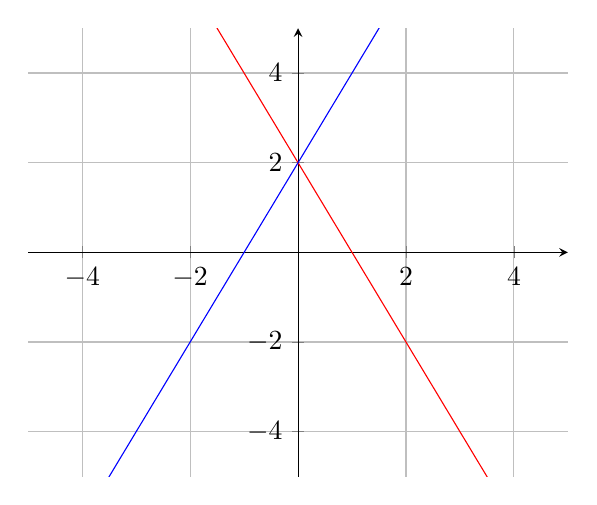
\begin{tikzpicture}
    \begin{axis}[xmin=-5, xmax=5, ymin=-5, ymax=5, axis x line=middle, axis y line=middle, grid=both]
    \addplot[domain=-5:5, color=red]{-2*x+2};
    \addplot[domain=-5:5, color=blue]{2*x+2};
    \end{axis}
    \end{tikzpicture} \\ 
\end{center}
\textbf{when extend to 3 dimensional space, situation become only intersect once with two planes} \\[5pt]
% ================================== 3 dimensional plane ===============================================
\tdplotsetmaincoords{70}{110} % I don't know why, but necessary
\begin{tikzpicture}[tdplot_main_coords,font=\sffamily]
\draw[-latex] (0,0,0) -- (4,0,0) node[left] {$x$};
\draw[-latex] (0,0,0) -- (0,4,0) node[below] {$y$};
\draw[-latex] (0,0,0) -- (0,0,4) node[left] {$z$};
\draw[fill=red,opacity=0.2] (-3,0,-3) -- (-3,0,3) -- (3,0,3) -- (3,0,-3) -- cycle;
\draw[fill=red,opacity=0.1] (-3,-3,0) -- (-3,3,0) -- (3,3,0) -- (3,-3,0) -- cycle;
\draw[thick](-3,0,0)--(3,0,0);
\node[anchor=south west,align=center] (line) at (3,3,3) {line of\\ intersection};
\draw[-latex] (line) to[out=180,in=75] (-2,0,0.05);
\end{tikzpicture}
\begin{tikzpicture}[tdplot_main_coords,font=\sffamily]
\draw[-latex] (0,0,0) -- (4,0,0) node[left] {$x$};
\draw[-latex] (0,0,0) -- (0,4,0) node[below] {$y$};
\draw[-latex] (0,0,0) -- (0,0,4) node[left] {$z$};
\tdplotsetrotatedcoords{45}{0}{0}
\begin{scope}[tdplot_rotated_coords]
\draw[fill=red,opacity=0.2] (-3,0,-3) -- (-3,0,3) -- (3,0,3) -- (3,0,-3) -- cycle;
\end{scope}
\tdplotsetrotatedcoords{90}{45}{0}
\begin{scope}[tdplot_rotated_coords]
\draw[fill=red,opacity=0.1] (-3,-3,0) -- (-3,3,0) -- (3,3,0) -- (3,-3,0) -- cycle;
\draw[thick](-3,{3/sqrt(2)},0) coordinate(x) --(3,{-3/sqrt(2)},0);
\end{scope}
\node[anchor=south east,align=center] (line) at (3,-1.5,3.5) {line of\\ intersection};
\draw[-latex] (line) to[out=0,in=135] (x);
\end{tikzpicture}
% ================================== 3 dimensional plane ===============================================

\subsection{Infinitely Many Solution}

\begin{center}
$\begin{vNiceArray}{cccc}[right-margin=.4em]
    1 & 2 & $-3$ & 1 \\ 
    0 & 1 & 5 & $-2$ \\
    0 & 0 & \color{red}0 & 0 \\
    \CodeAfter 
\end{vNiceArray}$ \\
\begin{center}
$\uparrow$\\
\color{red}z is not a leading variable. It is a free variable, meaning when z take different values, lines will change its slope and intersection with the coordinate, 
or plane will change inclination degree and intersection with coordinate, and so on for higher dimension 
\end{center}
\end{center}











\end{document}


